\section{Dati attività di verifica}
\subsection{Revisione dei requisti(RR)}
Al fine di presentare alla proponente i dati con la modalità a \textit{cruscotto informativo} le metriche verranno descritte attravero grafici evitando così uno stile torppo tabellare.
\subsubsection{Qualità di processo}
In questa sezione verranno analizzate le metriche e le valutazioni scaturite da esse.
\paragraph{Metriche dei processi}
\hspace{15cm}
Verranno presentate solo le metriche dei processi ISO utilizzate fino ad ora.
\begin{table}[]
	\resizebox{\textwidth}{!}{%
		\begin{tabular}{|l|l|l|l|}
			\hline
			\rowcolor[HTML]{34CDF9} 
			{\color[HTML]{333333} \textbf{Nome}} & {\color[HTML]{333333} \textbf{Valore ottenuto}} & {\color[HTML]{333333} \textbf{Commento}}                                                                                                                                         & {\color[HTML]{333333} \textbf{Voto}} \\ \hline
			Budget at competition                &                                                 & \begin{tabular}[c]{@{}l@{}}come si può notare\\ dal diagramma di gantt del ".."\\ sono stati raggiunti gli obiettivi\\ senza sforare il budget per questo\\ periodo\end{tabular} & ottimo                               \\ \hline
			Budget variance                      & 5\%                                             &                                                                                                                                                                                  & accettabile                          \\ \hline
			Cost variance                        & 0\%                                             & abbiamo utilizzato le ore prefissate, senza andare in debito                                                                                                                     & accettabile                          \\ \hline
		\end{tabular}%
	}
\end{table}
\paragraph{Maturità macro-processi ISO }
\hspace{15cm}
\begin{figure}[h!]
	\centering
	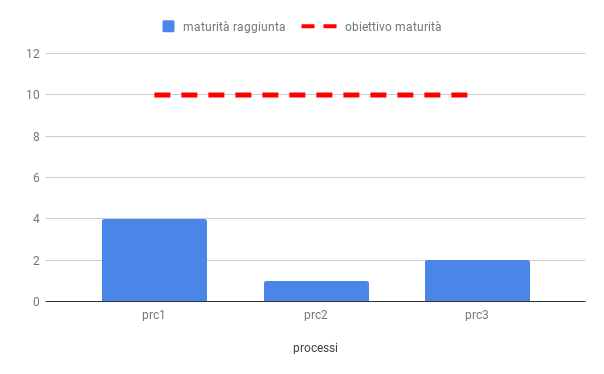
\includegraphics[scale=0.5]{MaturitaProcessi.png}
	\caption{Maturità macro-processi ISO 15504}
\end{figure}
\begin{itemize}
	\item \textbf{prc1:} processo gestito da automatismi, il gruppo sta imparando ad utilizzare quest'ultimi per rendere il lavoro più preciso e con meno possibilità di errore. Usando ad esempio toggle per il conteggio ore e integrazione slack con github tracciando le issue ha
	permesso di ottenere una migliore pianificazione;
	\item \textbf{proc2:} processo non ancora istanziato poichè non fa parte della revisione di requisit, abbiamo analizzato solo metriche in funzione degli obiettivi;
	\item \textbf{proc3:} processo non ancora istanziato, sarà comunque quasi completamente automatizzato
\end{itemize}
\subsubsection{Qualità di prodotto}
In questa fase ci si concentra principalmente sulla redazione dei documenti, pertanto le uniche metriche utilizzate sono quelle riguardanti i documenti.
Poichè, in particolari circostanze (non necessariamente rare), la valutazione automatica della leggibilità, se non tiene conto in alcun modo dei significati delle parole, può dare risultati inattendibili, per non dire fuorvianti si è scelto di non valutare i documenti tramite script che calcolano le metriche.
Nonostante cioò sono metriche puramente sintattiche, sono da considerare con la dovuta cautela \\
\url{https://docs.google.com/spreadsheets/d/1yMKJyV4I8FXQ7GUQOq8m1RdZeTYFTJ387ixzofNrfLI/edit?usp=sharing}
\url{https://www.webfx.com/tools/read-able/check.php?tab=Test+By+Url&uri=https%3A%2F%2Fwww.ispazio.net}
	 \\ \\
	Come si può notare dal trend dei grafici l'obiettivo è stato quasi sempre rispettato ottenendo dei documenti con una leggibilità media da istruzione superiore.
	\clearpage
\paragraph{Gunning Fog index}
\hspace{15cm}
\begin{figure}[h!]
	\centering
	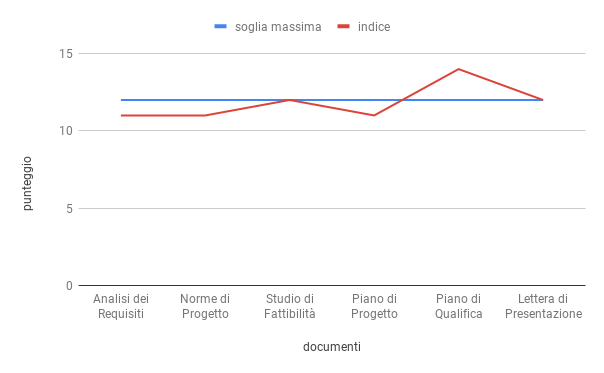
\includegraphics[scale=0.5]{GunningFogIndex.png}
	\caption{Gunning Fog index}

\end{figure}
%\clearpage
\paragraph{Simple Measure of Gobbledygook (SMOG)}
\hspace{15cm}
\begin{figure}[h!]
	\centering
	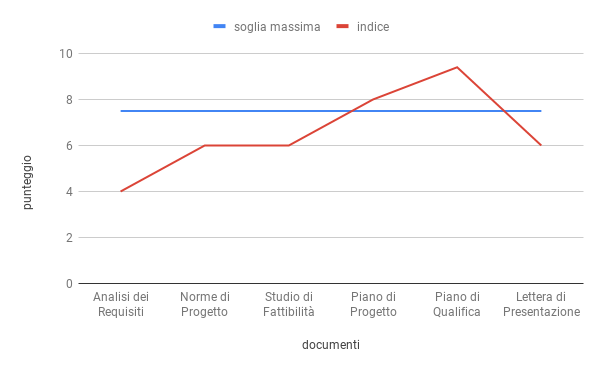
\includegraphics[scale=0.5]{Smog.png}
	\caption{SMOG}
\end{figure}
\clearpage
\paragraph{Gulpease Index}
\hspace{15cm}
\begin{figure}[h!]
	\centering
	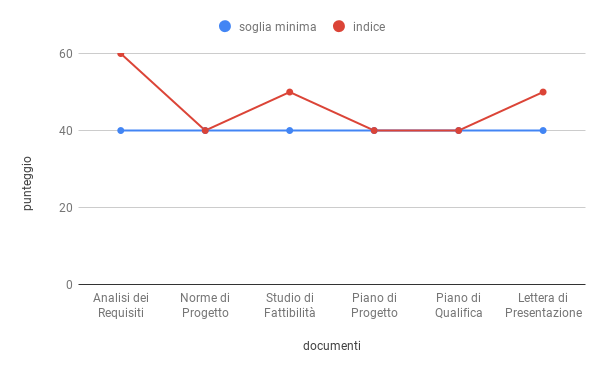
\includegraphics[scale=0.5]{GulpeaseIndex.png}
	\caption{Gulpease index}
\end{figure}

\paragraph{Errori sintattici}
\hspace{15cm}
 I verificatori hanno eliminato gli errori rimanenti presenti nei documenti, raggiungendo così il valore ottimale prefissato attraverso il software per il controllo ortografico presente in TexStudio. 
\subsubsection{Conclusioni}
Parlare se si è sforati nel budget (parlare quindi di metriche per il budget) e in quel caso perchè è successo.
\clearpage
\subsection{Revisione di Progettazione (RP)}
Questa sezione verrà riempita durante il periodo definito.
\subsection{Revisione di Qualifica(RQ)}
Questa sezione verrà riempita durante il periodo definito
\subsection{Revisione di Accettazione(RA)}
Questa sezione verrà riempita durante il periodo definito